\documentclass[./main.tex]{subfiles}

\begin{document}

Every node of the system consists of some components. The diagram in figure
\ref{fig:component_diagram} aims to provide an overview of all the components
of the world in which the application must work. Then there is a projection
over every component that belongs to the application server, where the internal
architecture and the information flow are described. Every functionality of the
application is strictly independent of the others; for this reason, every one
of them is fully exploited by a single (aggregated) component which is
represented with the same name of the functionality.\medskip\\
Components inside the database server are not described since their physical
implementation is not the core of this specification document. Components
outside the application server are not described since they cannot be modeled
by the developers. Components that interface with these external modules must
agree to the needed communication standards.

\begin{figure}[H]
\centering
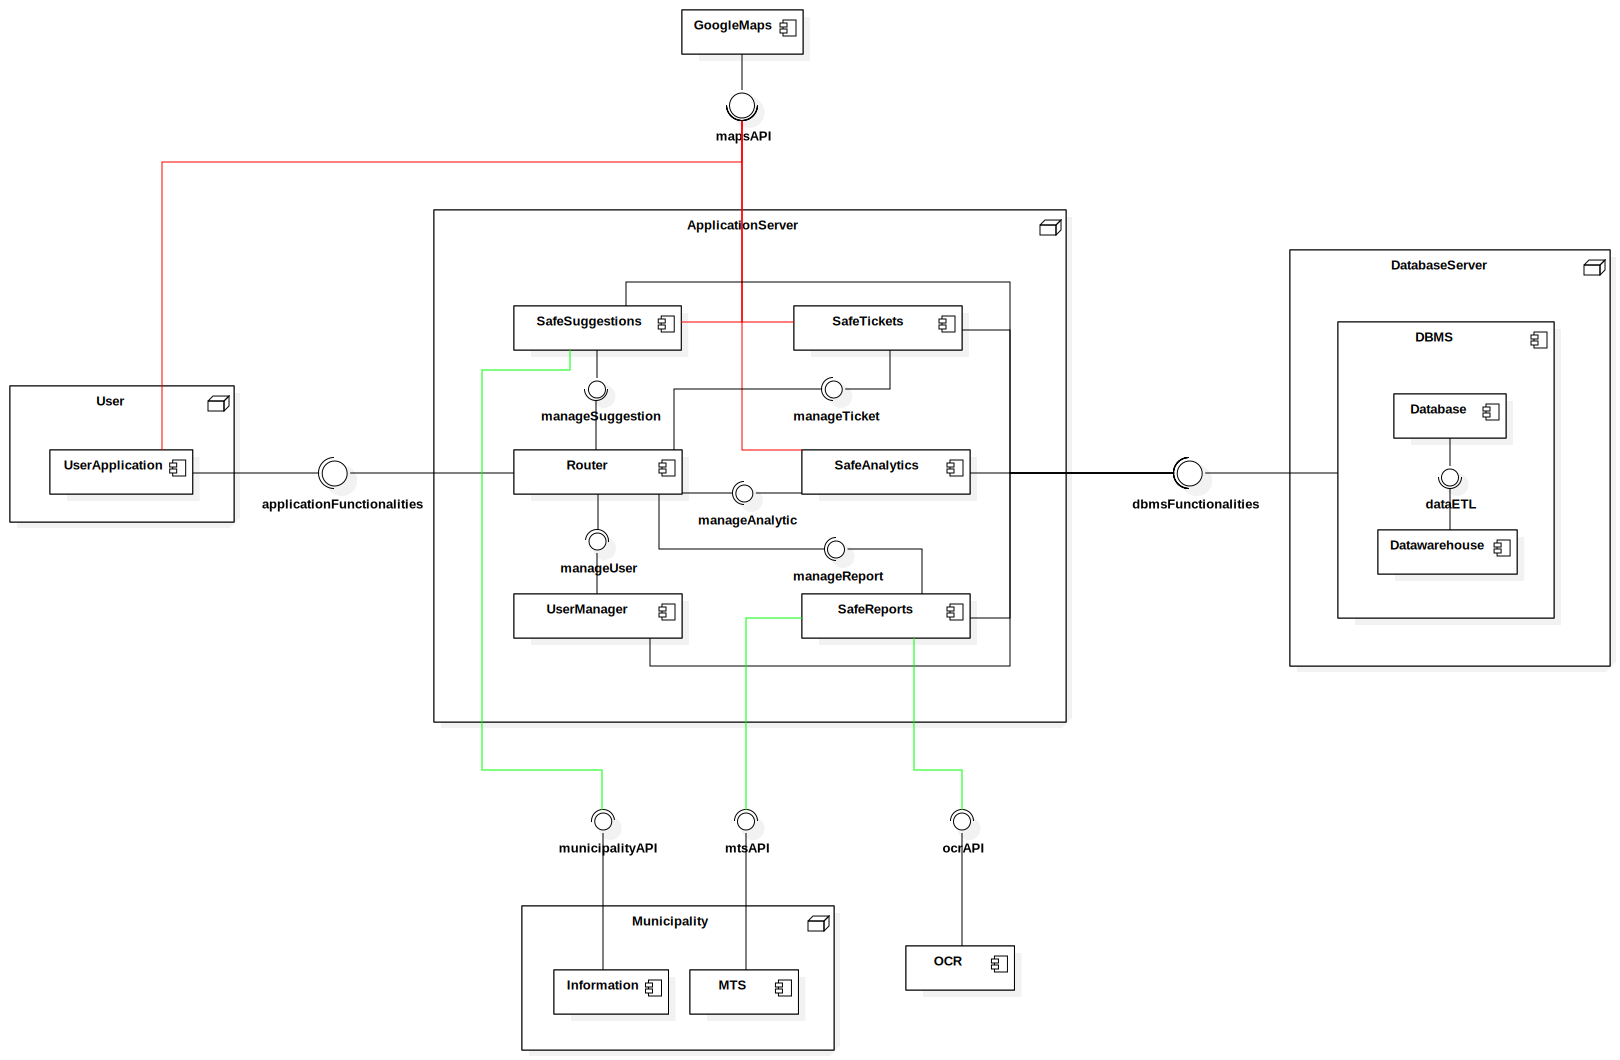
\includegraphics[width=\textwidth]{component_diagram}
\caption{Component diagram}
\label{fig:component_diagram}
\end{figure}

\begin{itemize}
\item
  \textbf{Router}\\
  Its purpose is to handle all the communications between the user and the
  application server. Using a specialized device to do this, minimizes the
  number of links between the client and the server. This involves a good level
  of scalability. The router manages all the messages, forwarding them to the
  responsible components. In particular, the router can recognize a user. This
  allows it to start the correct handling procedure on the correct component.
\item
  \textbf{UserManager}\\
  It is responsible for the user-related operation. It allows the user to login
  and to register, and eventually verifies the activation code during the
  signup procedure. It is not described in detail since it is not the core of
  the application.
  \begin{figure}[H]
  \centering
  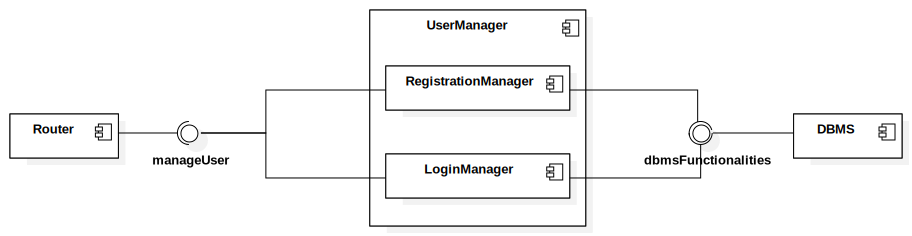
\includegraphics[width=\textwidth]{component_diagram_user_manager}
  \caption{UserManager component}
  \end{figure}
  \begin{itemize}
  \item
    \textbf{RegistrationManager} is responsible for the signup procedure.
  \item
    \textbf{LoginManager} is responsible for the login procedure.
  \end{itemize}
\item
  \textbf{SafeReports}\\
  It provides services to verify and store violation reports. It is split into
  several sub-components to avoid a centralized managing of communication with
  external tools. This involves better scalability since every component can be
  updated independently from the others.
  \begin{figure}[H]
  \centering
  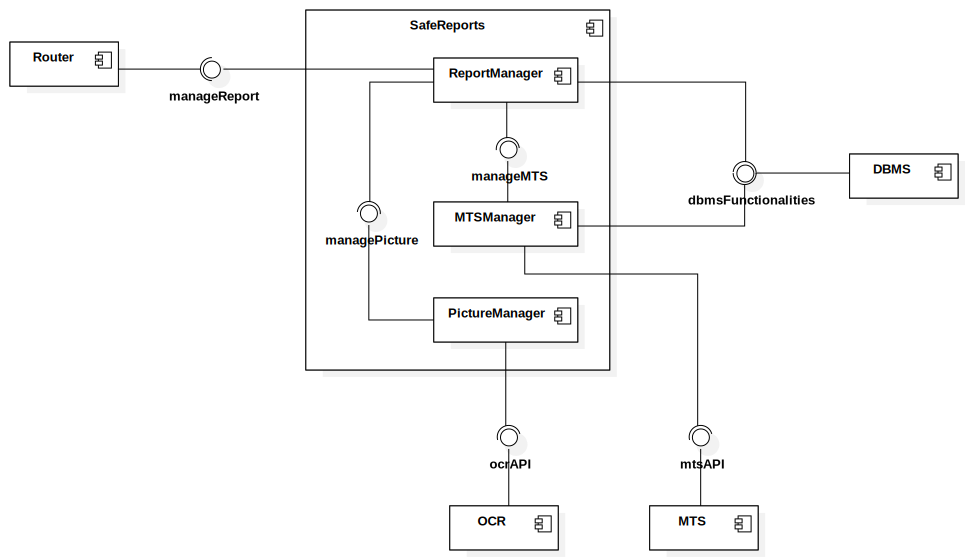
\includegraphics[width=\textwidth]{component_diagram_safe_reports}
  \caption{SafeReports component}
  \end{figure}
  \begin{itemize}
  \item
    \textbf{ReportManager} performs all the necessary integrity checks to
    ensure that the chain of custody has never been broken. When it receives a
    report, it forwards the image to \textbf{PictureManager} and waits for a
    response. If the picture is not good, it notifies the user that the
    procedure must be repeated. If the picture is good, it waits for a
    confirmation from the user. If the user confirms, the component asks the
    DBMS to store the report. The DBMS returns a value that determines if the
    report was not duplicated. If it wasn't, the component forwards the report
    to \textbf{MTSManager}.
  \item
    \textbf{MTSManager}\\
    It converts the reports in a suitable format for MTS and forwards them to
    the service. If a traffic ticket is generated, the ticket-related
    information answered by MTS is sent to the DBMS to be stored.
  \item
    \textbf{PictureManager}\\
    It manages the communication with the OCR software. It forwards the picture
    to the OCR and interprets the answer. Once it is done, it responds to
    \textbf{ReportManager}.
  \end{itemize}
\item
  \textbf{SafeAnalytics}\\
  It is just an interpreter between the application and the DBMS. It consists
  of a single component that directly interfaces with the external modules.
  \begin{figure}[H]
  \centering
  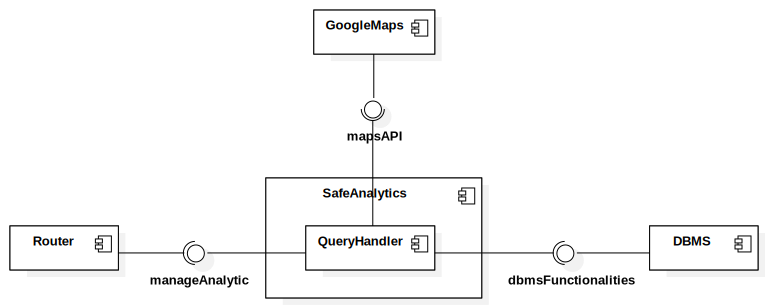
\includegraphics[width=\textwidth]{component_diagram_safe_analytics}
  \caption{SafeAnalytics component}
  \end{figure}
  \begin{itemize}
  \item
    \textbf{QueryHandler} receives the queries from \textbf{Router}. Once a
    query is received, the component checks that the selected filters are
    coherent with the access right of the user who made the query, since the
    component has unrestricted access to the DBMS. What happens is that
    \textbf{Router} calls a user-specific function in the interface provided by
    the query handler (the identification of the user is done by
    \textbf{Router}). Once the query is answered, the data are sent back to the
    user.
  \end{itemize}
\item
  \textbf{SafeTickets}\\
  Its behavior is the same as \textbf{SafeAnalytics}. The only difference is
  the format of the data the component works with.
  \begin{figure}[H]
  \centering
  \includegraphics[width=\textwidth]{component_diagram_safe_tickets}
  \caption{SafeTickets component}
  \end{figure}
  \begin{itemize}
  \item
    \textbf{QueryHandler} has the same behavior as the sub-component of
    \textbf{SafeAnalytics}. The only difference is that it doesn't need to
    check the validity of the filters since it offers his services only to
    authorities.
  \end{itemize}
\item
  \textbf{SafeSuggestions}\\
  It has the same purpose of \textbf{SafeAnalytics} and \textbf{SafeTickets}.
  Moreover, it manages the data extraction from the municipality information,
  periodically activating the update check. Then it forwards the data to the
  DBMS.
  \begin{figure}[H]
  \centering
  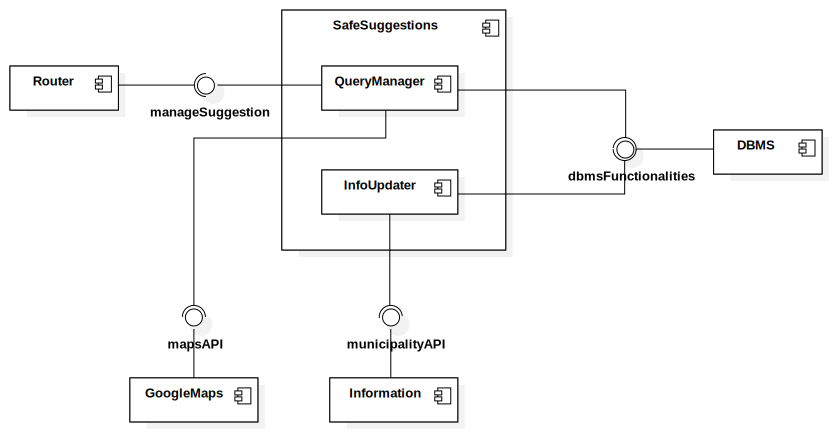
\includegraphics[width=\textwidth]{component_diagram_safe_suggestions}
  \caption{SafeSuggestions component}
  \end{figure}
  \begin{itemize}
  \item
    \textbf{QueryManager} works exactly as \textbf{QueryHandler}. Refer to that
    description.
  \item
    \textbf{InfoUpdater} is a sub-component that works independently from the
    others. Its purpose is to periodically check for the existence of new
    information from the municipality. If there is new information, it gets it
    and forwards it to the DBMS. The analysis of the extracted information is
    up to the database system.
  \end{itemize}
\end{itemize}

\end{document}